\appendix
\chapter{Solutions}
  \label{app:solutions}

  %% An alternative method to make this lists is with description environment
  %%
  %% \begin{description}
  %%   \item[Freezing media] \hfill \\
  %%     91\% FCS;
  %%     10\% DMSO
  %%   \item[Growth medium (HeLa)] \hfill \\
  %%     87\% DMEM;
  %%     10\% FCS;
  %%     1\% NEAA;
  %%     ...
  %% \end{description}

  %% The way we calculate the columns width (with eqparbox), doesn't work
  %% with memoir's ctabular so we are using longtable instead
  \begin{longtable}{>{\bfseries}\SolutionNameCol p{\dimexpr(\textwidth-\eqboxwidth{SolutionNameBox}-4\tabcolsep)}}
    \toprule
    Name & Recipe\\
    \midrule
    2YT broth               & \SI{16}{\g\per\l} tryptone;
                              \SI{10}{\g\per\l} yeast extract;
                              \SI{5}{\g\per\l}  NaCl.\\

    DMEM                    & \SI{4.5}{\g\per\l}   glucose;
                              \SI{110}{\mg\per\l}  L-glutamine;
                              \SI{584}{\ug\per\l}  sodium pyruvate;
                              \SI{15.9}{\mg\per\l} phenol red.\\

    DNA loading buffer (\SI{10}{\X}) & \pcent{25} Ficoll ($w/v$);
                              \SI{100}{\mM}      Tris--HCl pH=\num{7.4};
                              \SI{100}{\mM}      EDTA.\\

    FACS buffer             & \pcent{96} PBS ($v/v$);                   % 480.5 mL
                              \SI{2}{\mM} EDTA;                         % 2 mL
                              \SI{25}{\mM} HEPES buffer pH=\num{7.0};   % 12.5 mL
                              \pcent{1} FCS ($v/v$).\\                  % 5 mL

    Freezing media          & \pcent{90} FCS ($v/v$);
                              \pcent{10} DMSO ($v/v$).\\

    Growth medium (HeLa, HEp2) & \pcent{89}         DMEM ($v/v$);   % 500ml
                              \pcent{9}             FCS ($v/v$);    % 50ml
                              \SI{1}{\X}            NEAA solution;  % 5.5mL
                              \SI{50}{units\per\ml} penicillin;     % 5.5mL (Pen/Strep solution)
                              \SI{50}{\ug\per\ml}   streptomycin.\\ % 5.5mL (Pen/Strep solution)

    Growth medium (horse)   & \pcent{81}            DMEM ($v/v$);   % 500ml
                              \pcent{16}            FCS ($v/v$);    % 100ml
                              \SI{2}{\X}            NEAA solution;  %  12mL
                              \SI{50}{units\per\ml} penicillin;     % 5.5mL (Pen/Strep solution)
                              \SI{50}{\ug\per\ml}   streptomycin.\\ % 5.5mL (Pen/Strep solution)

    LB agar                 & \SI{20}{\g\per\l}  LB broth powder;
                              \SI{7.5}{\g\per\l} agar.\\

    LB broth                & \SI{20}{\g\per\l} LB broth powder.\\

    Ponceau S solution      & \pcent{5} Ponceau S ($w/v$);
                              \pcent{5} Acetic acid ($v/v$).\\

    Running buffer          & \SI{1}{\X}  TG;
                              \pcent{0.1} SDS ($w/v$).\\

    SSC (Saline Sodim Citrate) & \SI{150}{\mM} NaCl;
                              \SI{15}{\mM}     trisodium citrate.\\

    TAE (Tris Acetate EDTA) & \SI{40}{\mM} Tris;
                              \SI{20}{\mM} acetic acid;
                              \SI{1}{\mM}  EDTA.\\

    TBE (Tris Borate EDTA)  & \SI{89}{\mM} Tris;
                              \SI{89}{\mM} boric acid;
                              \SI{2}{\mM}  EDTA.\\

    TBS (Tris Buffered Saline)  & \SI{50}{\mM} Tris--HCl pH=\num{7.5};
                              \SI{100}{\mM}    NaCl.\\

    PBS-T (TBS-Tween)       & \pcent{99.95} PBS ($v/v$);
                              \pcent{0.05}  Tween 20 ($v/v$).\\

    TG (Tris Glycine)       & \SI{25}{\mM}  Tris;
                              \SI{192}{\mM} glycine.\\

    Transfer buffer         & \SI{1}{\X} TG;
                              \pcent{15} methanol ($v/v$).\\
    \bottomrule
  \end{longtable}


\chapter{List of plasmids}
  \label{app:plasmids}
  %% generate this automatically from SQlite db
  %% should we print the maps on genbank format, just the genbank features
  %% table, or a draw of the map, poiting to the database for the sequence
  %% details?

\chapter{List of primers}
  \label{app:primers}
  %% generate this automatically from SQlite db

\chapter{Documentation}
  \label{app:pod-doc}
  %% this setlist commands require the enumitem package and avoids that the very long item entries
  %% on the description environment (as it happens on the examples section), do not run out of the
  %% paper margins. See http://tex.stackexchange.com/questions/96267
  \setlist[description]{style=unboxed}
  \input{results/app-bp_genbank_ref_extractor-doc}
  \setlist[description]{style=standard}

\chapter{Structure and function of histone H2AX}
  \label{app:h2ax-review}

  The following manuscript was authored by David Miguel Susano Pinto and
  Andrew Flaus as part of this thesis studies. It was published in ``Genome
  Stability and Human Diseases'', Subcellular Biochemistry series, volume~50,
  2010.

  \documentclass[graybox]{svmult}

% choose options for [] as required from the list
% in the Reference Guide


\usepackage{mathptmx}       % selects Times Roman as basic font
\usepackage{helvet}         % selects Helvetica as sans-serif font
\usepackage{courier}        % selects Courier as typewriter font
\usepackage{type1cm}        % activate if the above 3 fonts are
                            % not available on your system
%
\usepackage{makeidx}         % allows index generation
\usepackage{graphicx}        % standard LaTeX graphics tool
                             % when including figure files
\usepackage{multicol}        % used for the two-column index
\usepackage[bottom]{footmisc}% places footnotes at page bottom
\usepackage{harvard}


% see the list of further useful packages
% in the Reference Guide

\makeindex             % used for the subject index
                       % please use the style svind.ist with
                       % your makeindex program

%%%%%%%%%%%%%%%%%%%%%%%%%%%%%%%%%%%%%%%%%%%%%%%%%%%%%%%%%%%%%%%%%%%%%%%%%%%%%%%%%%%%%%%%%

\begin{document}

\title*{Structure and function of histone H2AX}
% Use \titlerunning{Short Title} for an abbreviated version of
% your contribution title if the original one is too long
\author{David Miguel Susano Pinto   \and
        Andrew Flaus
}
\authorrunning{David Miguel Susano Pinto and Andrew Flaus}
\institute{Andrew Flaus
\at Centre for Chromosome Biology, Department of Biochemistry, National University of Ireland, Galway,
\email{andrew.flaus@nuigalway.ie}
}

\maketitle

\abstract{Histone H2AX is a histone variant found in almost all eukaryotes. It makes a central
contribution to genome stability through its role in the signaling of DNA damage events and by
acting as a foundation for the assembly of repair foci. The H2AX protein sequence is highly similar
and in some cases overlapping with replication-dependent canonical H2A, yet the H2AX gene and
protein structures exhibit a number of features specific to the role of this histone in DNA repair.
The most well known of these is a specific serine at the extreme C--terminus of H2AX which is
phosphorylated by Phosphoinositide--3--Kinase-related protein Kinases (PIKKs) to generate the
\ugamma H2AX mark. However, recent studies have demonstrated that phosphorylation, ubiquitylation
and other post-translational modifications are also crucial for function. H2AX transcript properties
suggest a capability to respond to damage events. Furthermore, the biochemical properties of H2AX
protein within the nucleosome structure and its distribution within chromatin also point to features
linked to its role in the DNA damage response. In particular, the theoretical inter-nucleosomal
spacing of H2AX and the potential implications of amino acid residues distinguishing H2AX from
canonical H2A in structure and dynamics are considered in detail. This review summarises current
understanding of H2AX from a structure--function perspective.}

\keywords{Histone, H2AX, structure--function, chromatin structure, DSB, DNA repair}

\begin{description} [snRNA]
 \item[DSB] Double Strand Break
 \item[DDR] DNA Damage Response
 \item[HDE] Histone Downstream Element
 \item[HR] Homologous Recombination
 \item[IR] Ionising Radiation
 \item[NHEJ] Non-Homologous End Joining
 \item[PIKK] Phosphoinositide--3--Kinase-related protein Kinase
 \item[PTM] Post-Translation Modification
 \item[SHL] SuperHelical Location
 \item[SLBP] Stem--Loop Binding Protein
 \item[snRNA] small nuclear RNA
 \item[TSS] Transcription Start Site
\end{description}

\newpage

\section{Introduction}

\label{sec:introduction}
Maintenance of the genome stability is of great importance to all organisms because DNA damage can
have serious biological implications including genetic disorders and cancer \cite{PJM07}. One
mechanism for maintaining genome stability is to increase DNA repair \cite{CLKWK98} and an important
paradigm for DNA repair is the mechanism for identifying and facilitating re-ligation of DNA Double
Strand Breaks (DSBs). DSBs are one of the most serious forms of DNA damage because they involve loss
of genetic continuity. They arise from a variety of causes including not only the action of DNA
damaging agents but also normal functions such as meiosis and antibody class switching. An important
player in the DNA Damage Response (DDR) for dealing with DSBs is the histone variant H2AX, which is
an integral component of the chromatin packaging of eukaryotic genomes.

\subsection{Chromatin Structure and Genome Stability}
\label{subsec:genome-stability}
Eukaryotic DNA is not dispersed randomly within the cell nucleus. Instead, it is packaged into the
chromatin structure which compacts DNA and organises accessibility to the genome. This chromatin
packaging is hierarchical, based on the nucleosome as a fundamental building block. The canonical
nucleosome comprises two copies of each core histone (H2A, H2B, H3 and H4) around which 147\,bp of
DNA is wound in a superhelical spiral \cite{CAD+02}. The nucleosomes are connected by short DNA
linkers to form repeating units which subsequently arrange in a number of higher-order structural
levels up to condensed metaphase chromosomes.

Despite its modular structure, the arrangement of chromatin is not static and must be ``remodeled''
during nuclear processes including DNA repair. This remodeling is driven by two general mechanisms:
Firstly, molecules such as ATP-dependent remodelers and chromatin-binding proteins can directly
modify the structure. Secondly, physiochemical properties of chromatin can be modulated by
post-translational modification or insertion of histone variants to alter its stability \cite{GFMG03,JA06}.

\subsection{H2AX and DNA repair}
\label{subsec:H2AX-repair}
H2AX and another histone variant, H2A.Z, were both identified in human cells by their different
migration compared to canonical H2A isoforms on SDS and acetic acid--urea gels \cite{MHPW80}. In
this separation, H2AX and H2A.Z were two of four unidentified species arbitrarily labeled T, W, X
and Z\@. Subsequently, it was found that T and W were the ubiquitylated forms of X and Z \cite{MHPW80}.
H2A.Y is an alternative name for macroH2A1. Although originally labeled as H2A.X, the internal
period (`\,.\,') separating the X has fallen into disuse so the H2AX name is almost universally used
in the DNA repair field. In contrast, the internal period has historically been retained in H2A.Z,
whose major roles have been subsequently associated with transcription \cite{JA06}.

A distinct function for H2AX was uncovered some 18 years after its initial identification when human
and mouse serine 139 was observed to be rapidly phosphorylated in response to treatments that cause
DSBs \cite{EPR+98}. In structural nomenclature, the phosphorylation occurs on the serine oxygen in
the gamma position so the modified form is widely referred to as \ugamma H2AX\@. This \ugamma H2AX
phosphoprotein is found to be rapidly concentrated around DSBs in centers termed ``foci'' that can
extend for a range of up to 2\,Mbp away from the damage site \cite{EPR+99}.

The amino acid region surrounding serine 139 matches the consensus recognition sequence for a set of
PhosphoInositide--3--Kinase-related protein Kinases (PIKKs) known to be central in the DNA damage
response from genetic studies in yeast \cite{JAD00}. The link between PIKKs and \ugamma H2AX
formation has been directly demonstrated by biochemical inhibition using mutagenesis in yeast \cite{JAD00}
and wortmannin in higher cells \cite{TTP+00}.

\ugamma H2AX is a widely recognised participant in DSB repair and is one of the earliest markers of
damage \cite{DRP+03}. Other DNA repair-related proteins subsequently congregate at the \ugamma H2AX
foci during the repair process. Although their recruitment to DSBs is not completely dependent on
H2AX phosphorylation, H2AX is an important element in proper damage response foci formation by
enhancing the retention of repair factors after their initial recruitment \cite{ACOF+03}.
H2AX$^{-/-}$ mice have moderate defects including radiation sensitivity, growth retardation and
immunodeficiency which are consistent with deficiencies in DNA repair \cite{ACSP+02,ACSD+03}.
Importantly, these phenotypes are only moderate and suggest redundancy for the role of H2AX\@. Nevertheless,
karyotypes of H2AX-deleted genomes also reveal a high number of translocations and chromosome
rearrangements directly demonstrating increased genomic instability.

\section{Structural Properties of H2AX}
\label{sec:structure-properties}
Based on the linkage between the early H2AX phosphorylation event and the DDR, a large number of
studies have focussed on \ugamma H2AX and its subsequent interactions with the repair mechanism.
Less consideration has been given to the biochemical properties of H2AX itself.

H2AX is one of a set of histone H2A proteins encoded in eukaryotic genomes, the human genome holding
21 genes of H2A forms. The canonical human H2A has two biochemically separable isoforms, H2A.1 and
H2A.2. No functional difference between those isoforms is known, and the basis of their distinction
appears to be dependent on residue 51 encoding, respectively, either a leucine or methionine despite
further heterogeneity within each isoform \cite{DBMC+06,WFM+02}. Four additional H2A variants with
distinct functions are encoded in humans and other higher eukaryotes: H2AX, H2A.Z, macroH2A1,
macroH2A2, H2A.F/Z and H2ABbd \cite{WFM+02}.

\subsection{Definition of H2AX}
\label{subsec:relation-H2A-H2AX}
The H2AX variant is principally defined by the capacity to accept phosphorylation on a serine near
the C--terminus through the activity of PIKKs such as ATM, ATR and DNA-PK on the consensus motif
SQ[E/D]$\varPhi$ (where $\varPhi$ is a hydrophobic residue). The number of residues separating this
motif from the core histone fold region is variable and has been claimed to correlate with the
evolutionary complexity of the organism \cite{CRDP+02}. For example, the spacing of 29 residues
between the end of the H2AX \ualpha 3 helix and the phospho serine in \emph{Saccharomyces cerevisiae}
and \emph{Giardia lamblia} is 12 residues shorter than in humans and mice.

In higher eukaryotes, H2AX is encoded as a separate histone variant of H2A but in lower organisms
such as \emph{S.\ cerevisiae}, \emph{G.\ lamblia} and certain protists, the distinguishing H2AX
features are merged into the canonical H2A \cite{HSM03,SJN06} so that the canonical H2A also acts as
the H2AX variant. In \emph{Drosophila melanogaster}, the H2AX feature is instead merged with H2A.Z
as a single variant, H2AvD, that is distinct from the canonical H2A \cite{MCG02}.

Based on phylogenetic analysis, it has been suggested that H2AX appeared multiple times in
eukaryotes as an example of parallel evolution \cite{HSM03}. However, the differences between
metazoan H2AX and canonical H2A sequences are few in number and this could be confounding to
phylogenetic algorithms. An alternative hypothesis is that the  H2AX function is ancestral and
canonical H2A evolved from the H2AX when complete phosphorylation became unnecessary or undesirable
as genomes expanded. This would explain the preeminence of the H2AX variant in \emph{G.\ lamblia}
and \emph{S.\ cerevisiae} compared to the lower abundance in mammals.

It has remained something of a puzzle that no H2AX variant function is identifiable in
\emph{Caenorhabditis elegans} \cite{HSM03} or some protists \cite{SJN06}. A search of all predicted
\emph{C.\ elegans} histones protein sequences reveals no PIKK consensus motifs in the coding
sequence or in any frame downstream of the annotated stop codons for any of the core histone genes
(data not shown). However, the related \emph{C.\ briggsae} genome contains the motif SQDY within the
\mbox{cpar--1} isoform of \mbox{CENP--A}, the centromeric \mbox{H3-like} histone. Alignment of seven
known \emph{Caenorhabditis} \mbox{CENP--A} homologues shows that this motif is quite conserved, with
the sequence being SSDL in \emph{C.\ elegans} \mbox{cpar--1} (Fig.\ \ref{fig:celegans}). Although
these do not strictly conform to the classic PIKK recognition site sequence, non-canonical sites are
known to be recognised by them\cite{SYC+05}.

This potential merger of H2AX with \mbox{CENP--A} is interesting for several reasons: Firstly,
\emph{C.\ elegans} utilises holocentric chromosomes so \mbox{cpar--1} is thought to be distributed
throughout the genome \cite{MMH+05}. Secondly, \mbox{cpar--1} appears to be more weakly expressed
than the other \mbox{CENP--A} homologue in the \emph{C.\ elegans} genome, \mbox{hcp--3} \cite{MMH+05},
recalling the H2AX/H2A ratio in human and mouse chromatin. Finally, the SQDY/SSDL motif is located
at small 3--4 residue insertion unique to the core histone fold of \mbox{CENP--A} family proteins.
This insertion immediately abuts lysine 79 of canonical H3 which is also implicated in the DDR
(Fig.\ \ref{fig:celegans})\@. \mbox{CENP--A} family proteins do not have lysine at the equivalent of
position 79 of canonical H3.

\subsection{H2AX Gene}
\label{subsec:H2AX-gene}
Canonical histone genes in humans are spread over one large and two small clusters named HIST1,
HIST2 and HIST3. These are located at 6p21--p22, 1q21 and 1q42 respectively (Table~\ref{tab:H2A-localisation}).
Canonical H2A is encoded by sixteen genes, twelve of which are located in HIST1, three in HIST2 and
one in HIST3. H2A variants are located outside these histone clusters in the human genome, with the
H2AX--encoding gene H2AFX at 11q23.2--11q23.3 \cite{IZP+94} (Table~\ref{tab:H2A-localisation}).
Histone variant gene names typically include the letter F for family.

The H2AFX promoter region, 151\,bp upstream from the transcription start site, shows higher activity
than the typical canonical H2A.1 HIST1H2AE promoter in transcription reporter assays \cite{VSI94}.
There are two CCAAT elements upstream of the TATA box in H2AFX (Fig.~\ref{fig:H2AFX}) compared to a
single CCAAT element in the H2A.1. The CCAAT element proximal to the TATA box in H2AFX has a
significant effect on expression, whereas this element has no apparent effect on promoter activity
in the canonical H2A promoter. The transcription factors that bind to the element also bind to the
distal CCAAT as well as to three similar elements in H2AFZ but not to the one in the H2A.1 promoter \cite{VSI94}.
This suggests that H2AFX is regulated independently of canonical H2A.

\subsection{H2AX Transcripts}
\label{subsec:H2AX-transcripts}
A fundamental distinction between histone types is whether their expression is replication-dependent
or replication-independent. This difference is a consequence of the requirement for large amounts of
canonical histones during S~phase to package the newly duplicated genome (i.~e.\ replication-dependence).
In contrast, variant or ``replacement'' histones often appear to be inserted into chromatin to replace
canonical histones for functional reasons throughout the cell cycle and are therefore replication-independent \cite{WFM+02}.

Canonical histone genes lack introns, probably to circumvent the requirement for primary transcript
processing when histones must be rapidly produced at S~phase. A number of transcript features appear
to enhance the capacity of replication-dependent histone expression by up to 35-fold during S~phase.
In fact, there is only a five-fold increase in their transcription rate at S phase, compared to the
other phases of cell cycle so regulation acts strongly at the post-transcriptional level \cite{MEH+91}.
Replication-dependent histone transcripts lack a poly(A) tail and encode a stem--loop followed by a
purine-rich Histone Downstream Element (HDE) downstream of the stop codon. The stem--loop interacts
with the Stem--Loop Binding Protein (SLBP) to stabilise the mRNA in S~phase \cite{MLW+00} while the
HDE interacts with U7~snRNA to direct  efficient 3' end processing \cite{GB85}.

Human H2AX transcripts exhibit characteristics of both replication-dependent and replication-independent
histones. The H2AFX gene lacks introns, and has two alternative transcripts: one shorter form contains
the characteristic stem--loop, and the other longer form contains a downstream poly(A) tail \cite{CMWMB89}
(Fig.~\ref{fig:H2AFX}). The combined synthesis of H2AX transcripts has been described as ``weakly
replication-linked at best'' since the H2AFX promoter keeps the levels of both transcripts high
through the cell cycle \cite{VSI94}. However, the cell cycle linkage of the forms is unclear and no
study has reported the effect of DNA damage on transcription levels.

\subsection{H2AX Protein}
\label{subsec:H2AX-protein}
Despite the large amount of attention paid to the DNA damage-linked serine phosphorylation by PIKKs,
the H2AX protein itself has a number of additional unique properties.

The defining feature of H2AX is considered to be the C--terminal region with the SQ[E/D]$\varPhi$ motif
(Fig.~\ref{fig:H2AX-logo}). As mentioned in Sect.~\ref{subsec:relation-H2A-H2AX}, the number of
residues separating this motif from the histone fold is variable and claimed to correlate with the
evolutionary complexity of the organism \cite{CRDP+02}. The residues responsible for this variable
spacing are mainly hydrophilic with a high glycine and proline content suggesting a flexible,
unstructured nature so the basis for the correlation could be more directly related to a structural
constraint such as the variation in internucleosomal repeat lengths of organisms which itself shows
linkage with evolutionary complexity.

In addition to the C--terminal motif, amino acid residues 6, 16, 38 and 99 of H2AX are different
from the human H2A.1 consensus (Figs.~\ref{fig:H2AX-logo} and~\ref{fig:H2AInNucleosome}). Inspection
of the human and \emph{X.\ laevis} histone based nucleosome structures reveals that H2A residue~6 is
located in the flexible N--terminal tail and residue~16 is located at the very base of the tail
(Figs.~\ref{fig:H2AInNucleosome} and~\ref{fig:framed}b) which tracks the minor groove at superhelical
location~4.5 (SHL4.5) (Fig.~\ref{fig:framed}a). The substitution of glutamine with threonine at
position~6 in H2AX introduces a potential hydroxyl site for post-translational modification that is
not present for the glutamine in canonical H2A. In contrast, the threonine to serine substitution
conserves the modifiable hydroxyl at position~16.

Asparagine~38 is located in the loop between the \ualpha 1 and \ualpha 2 helices of H2A within the
nucleosome (Figs.~\ref{fig:H2AInNucleosome} and~\ref{fig:framed}c). Importantly, this residue makes
direct contact with the equivalent amino acid in the other H2A--H2B dimer in the nucleosome structure
and has been suggested to affect both nucleosome stability and the balance between homotypic and
heterotypic combinations (see Sect.\ \ref{subsec:H2AX-distribution}) of H2A types within the yeast
nucleosome \cite{CLW01}. It is possible that the change of residue~38 from asparagine in H2A to
histidine in H2AX could also affect nucleosome stability and dynamics. For example, weakening of
interactions between the two H2A-H2B histone fold dimers could result in increased nucleosome
flexing and impact the ability to condense into stable higher order chromatin structure. Furthermore,
the presence of the histidine in H2AX could affect the stabilisation of a second copy of H2AX
relative to canonical H2A within the nucleosome. This change of asparagine to histidine at
position~38 occurs only in higher organism H2AX and could potentially drive a bias towards either
homotypic H2AX-only or heterotypic H2AX--H2A mixed nucleosomes which could have consequences for the
distribution of H2AX in chromatin (see Sect. \ref{subsec:H2AX-distribution}).

The effect of the final substitution distinguishing canonical H2A and H2AX where lysine becomes
glycine at position~99 is less clear. This residue is located in a sharp turn immediately after
the \ualpha 3 helix and points towards the C--terminal ends of H3 and H4 but makes no direct
interactions in the nucleosome (Figs.~\ref{fig:H2AInNucleosome} and~\ref{fig:framed}d). Nevertheless,
the exchange of the large, positively charged and potentially modifiable lysine for the highly
flexible glycine in H2AX could potentially alter stability and flexibility of the nucleosome.

\subsection{H2AX Post-Translational Modifications}
\label{subsec:H2AX-PTM}
Histones typically have a large proportion of amino acid residues which are modified post-translationally
for functional reasons so it is significant that three of the four residues distinguishing human H2A
and H2AX in the core region are capable of distinction via post-translational modification
(i.~e.\ Thr\,6 and Ser\,16 in H2AX vs.\ Thr\,16 and Lys\,99 in canonical H2A).

However, only the phosphorylation of H2AX serine 139 by PIKKs in response to DNA damage has been
intensively studied. This modification has been demonstrated to enhance access of restriction
enzymes and DNA methylases to the DNA, possibly by reducing nucleosome stability \cite{KHHK+08}. In
the same study the activity of the FACT complex which can facilitate dissociation of H2A/H2B dimers
from nucleosomes was shown to increase after H2AX phosphorylation.

One of the most recently reported post-translational modifications of H2AX related to DSB is the
phosphorylation of tyrosine~142 in the PIKK recognition motif of human H2AX \cite{XLS+09,CJT+09}. In
contrast to the phosphorylation of Ser\,139, this Tyr\,142 residue is phosphorylated under normal
conditions with DNA damage acting as trigger for its dephosphorylation. The dephosphorylation seems
to not only precede the phosphorylation of Ser\,139, but also to be a prerequisite for the Ser\,139
phosphorylation. When Tyr\,142 is phosphorylated, affinity of Ser\,139 to the DNA damage response
factors MDC1, MRE11 and Rad50 is greatly reduced and binding by pro-apoptopic factor JNK1 was found
to occur instead. It has therefore been suggested that the phosphorylation status of Tyr\,142 is a
determinant of cell fate after DNA damage.

H2AX can also be subject of acetylation at lysine~5 \cite{PB81} and to both mono- and poly-ubiquitylation
at lysine~119 dependent on the prior acetylation at Lys\,5 (Table~\ref{tab:H2AX-PTM}) \cite{ITK+07}. These
modifications are intimately related to DNA repair because their levels increase significantly after
exposure to DSB-inducing Ionising Radiation (IR) and appear to drive H2AX eviction from the nucleosome
by the action of Tip60 complex and UBC13 \cite{ITK+07}. However, conflicting data about the
interdependence of these effects with phosphorylation has recently been reported \cite{RVD+09}.

Other modifications unrelated to DNA damage have been reported for H2AX, including a rather unusual
biotinylation of Lys\,9 and Lys\,13 \cite{CCK+06} and the phosphorylation of Ser\,1 \cite{PB81}. By
homology to canonical H2A, it is probable that Lys\,9 and Lys\,13 can also be acetylated \cite{ZEP+03}
and Thr\,120 phosphorylated \cite{ANY+04}. Another interesting possible post-translational modification
is a methylation at Lys\,127 \cite{ZEP+03}. Although it was inconclusive whether Lys\,125 or Lys\,127
is the target of this methylation, it is tempting to speculate that it occurs at Lys\,127 since this
residue is the only one conserved in the C--terminal of all human H2A sequences (Fig.~\ref{fig:H2AX-logo}).

\subsection{H2AX Distribution in Chromatin}
\label{subsec:H2AX-distribution}
The original estimates of H2AX abundance in human cells reported cell line specific values from
2.5--25\% of total H2A in asynchronous immortalised cell lines \cite{EPR+98}. These values were
determined by densitometry of Coomassie-stained, acid-extracted histones in two-dimensional gels. A
10\% abundance value of H2AX has become accepted despite wide differences in the study and the fact
that HeLa cells were reported to contain 2.5\% H2AX\@.

Although it is tempting to interpret 10\% abundance as implying every tenth nucleosome will contain
H2AX, combinatorial features of nucleosomes make the statistics of spacings between H2AX occurrences
in the chromatin fibre more complex. H2AX can be incorporated either as one or as two copies per
nucleosome (Fig.~\ref{fig:H2AX-distribution}A), and the H2AX-containing nucleosomes can be either
randomly or non-randomly distributed along the chromatin fibre (Fig.~\ref{fig:H2AX-distribution}B--C).
Random incorporation would lead not simply to each tenth nucleosome containing H2AX, but to a
geometric distribution of spacings between H2AX-containing nucleosomes. This predicts many instances
of small spacings and some instances of very large spacings, and has clear implications for the
ability of \ugamma H2AX to signal local damage events as well as for the spreading of the
phosphorylation along the chromatin fibre.

\subsubsection{Combinatorial potential in H2AX distribution}
\label{subsubsec:Combinatorial-potential}
The combinatorial potential for H2AX inclusion has two separate features which could affect the
detailed distribution of H2AX along chromatin.

Firstly, either one or two H2AX polypeptides can in principle be present within a nucleosome: Two
H2AX copies would give rise to a ``homotypic'' H2AX/H2AX (`XX') nucleosome, whereas a single H2AX
copy will give rise to a ``heterotypic'' H2AX/H2A (`XA') nucleosome (Fig.~\ref{fig:H2AX-distribution}A).
It is currently unknown whether there is a bias for either homotypic or heterotypic nucleosomes
(see Sect.~\ref{subsec:H2AX-protein}) although this affects the statistics of H2AX spacing in
chromatin since the XA combination yields twice as many H2AX-containing nucleosomes than XX for a
given H2AX abundance.

Secondly, the spacing of nucleosomes containing H2AX should have a major influence on its functional
roles in DSB signaling, assembling of repair foci and facilitating the repair machinery. H2AX
nucleosomes could be randomly distributed (Fig.~\ref{fig:H2AX-distribution}B) or subject to clustering
in one (Fig.~\ref{fig:H2AX-distribution}C) or three dimensions (Fig.~\ref{fig:H2AX-distribution}D). Any
mechanism randomly assembling chromatin from pools of XX and/or XA versus canonical H2A--H2A (`AA')
nucleosomes will give rise to a geometric distribution of spacings between H2AX (Fig.~\ref{fig:H2AX-graphs}A).
This distribution predicts a bias towards small spacings (Fig.~\ref{fig:H2AX-graphs}A).

\subsubsection{Simulation of random H2AX inclusion}
\label{subsubsec:Simulation-random}
Simple computational simulations reveal interesting features in this H2AX spacing distribution. In
the simplest case of H2AX assembling in a mixture of XA and XX nucleosomes, 10\% overall H2AX
abundance would generate an average of 4.3 nucleosomes between H2AX occurrences along the chromatin
fibre (Fig.~\ref{fig:H2AX-graphs}B). The mean spacing is highly sensitive to H2AX abundance
(Fig.~\ref{fig:H2AX-graphs}A), so 2.5\% and 25\% H2AX abundances yields means of 19.3 to 1.3
nucleosomes, respectively (Fig.~\ref{fig:H2AX-graphs}B). Similar results arise for calculations
where only heterotypic XA nucleosomes can assemble and homotypic XX nucleosomes are structurally
precluded. In contrast, if heterotypic XA nucleosomes are precluded and only XX nucleosome
structures can assemble, then 10\% H2AX abundance yields a mean spacing of 9 nucleosomes between
H2AX occurrences. The mean spacings for 2.5\% and 25\% H2AX abundance are 39 to 3 nucleosomes
respectively (Fig.~\ref{fig:H2AX-graphs}B).

\subsubsection{Functional implications of H2AX distribution}
\label{subsubsec:Functional-impliactions}
These simple models of random nucleosome incorporation have interesting implications. The occurrence
of occasional large H2AX spacings could limit both processive \ugamma H2AX spreading along the
chromatin fibre and the proximity of H2AX in solenoidal higher order chromatin packaging. At 10\% H2AX
abundance, 23\% of nucleosomes in mixed XA and XX nucleosomes will be spaced by more than 6 nucleosomes
and in the extreme case of 2.5\% H2AX abundance, 84\% of solely homotypic XX nucleosomes would be
spaced by more than 6 nucleosomes.

This sensitivity of H2AX spacing in chromatin to abundance provides a potential opportunity for the
cell to regulate responsiveness to damage. For example, if H2AX expression is up-regulated the mean
proximity of randomly inserted H2AX will rapidly increase and effects such as processive \ugamma H2AX
spreading and retention of DDR factors at foci will be significantly enhanced.

It is unknown whether H2AX distribution varies between euchromatin and heterochromatin. However,
differences in H2AX response have been reported according to the condensation level of chromatin and
phosphorylation of Ser\,139 has been observed to occur preferentially in euchromatin \cite{IGC+07}.
This preference is overcome during replication of heterochromatin when it is in a less condensed
state \cite{IGC+07}. The distinction between active and inactive chromatin can also be regulated, as
demonstrated for phosphorylation of KAP--1 by ATM reducing the access of DNA repair proteins to
heterochromatic regions of the genome \cite{AAG+08}.

\subsubsection{Possibility of non-random H2AX distribution}
\label{subsubsec:Nonrandom-distribution}
If H2AX nucleosome incorporation is not a random process (Fig.~\ref{fig:H2AX-distribution}B),
inhomogeneity could also exist at a more local level. For example, small ``islands'' of higher
density H2AX nucleosomes could be interspersed within broader regions with lower relative abundance
of the variant (Fig.~\ref{fig:H2AX-distribution}C). A recent study using a novel high-resolution
microscopy observed several thousand small spatial clusterings of H2AX and pointed to a mutual
exclusivity of H2AX and the phosphorylated form \cite{JBBTB06}. This would be consistent with a
clustering model (Fig.~\ref{fig:H2AX-distribution}D) that enhanced the kinetics of the damage
signaling at foci, perhaps by making use of a chromatin structural feature such as the chromosomal
scaffold \cite{JBBTB06}. The inherent clustering and active insertion of H2AX in the DDR could also
drive larger scale chromosomal rearrangements through chromatin stability (Fig.~\ref{fig:H2AX-distribution}D) \cite{KHHK+08}.

\section{Functional Roles of H2AX}
\label{sec:function}
Phosphorylation of H2AX serine 139 by PIKKs to generate ``\ugamma H2AX foci'' is an early and
characteristic feature of DSB events. This modification is thought to be the primary identifier of
the location of DNA damage and would therefore be central to the function of H2AX.

The \ugamma H2AX foci extend for 2--30\,Mbp along the chromatin fibre \cite{EPR+99}, implying the
involvement of a span of 10$^4$--10$^5$ nucleosomes per individual DSB repair event. At 10\% H2AX
abundance, this would involve up to 10$^2$--10$^4$ H2AX molecules and hence a 10$^2$--10$^4$ fold
amplification of DSB event signal. A direct link between the site of a lesion and a single focus has
been observed \cite{KRIK+03}, suggesting that there is a linkage between \ugamma H2AX and the repair
mechanism. Many protein factors have been identified, which depend directly or indirectly on the
phosphorylation of H2AX at serine 139. Thereafter, it appears to act as a foundation for recruitment
of DDR factors at DSB sites \cite{TTP+00}. As a consequence, H2AX performs a role in both localisation
and structuring of the repair focus.

\subsection{Initiation of H2AX Phosphorylation as a Reporter of DSB Events}
\label{subsec:H2AX-reporter}
The process of establishing H2AX phosphorylation at the characteristic terminal motif can be performed
by any of the three PIKKs ATM, ATR and DNA--PK\@. Their induction and binding characteristics suggest
that H2AX phosphorylation for focus generation can be distinguished by an initiation phase when a
small number of phosphorylations are made at nucleosomes adjacent to the break, and a spreading phase
in which a larger region of phosphorylation extends one-dimensionally from either side of the break.
The structural exposure of the serine 139 site through chromatin flexibility will be crucial determinant
of the modification event (see Sect.\ \ref{subsec:H2AX-PTM}).

ATM has been considered a strong candidate as the principal kinase responsible for the initiation phase
of general damage events because it responds to changes in chromatin conformation expected when a
spontaneous DSB event releases local superhelical tension \cite{CJB03}. ATR appears to be linked to
replication stress or UV damage events which lead to breaks as indirect consequences, so ATR is recruited
by ATRIP which detects single-stranded DNA\@. DNA--PK is localised to DSBs in complex with the end-binding
protein Ku, so such an association will act to limit the distance from the damaged end on which DNA--PK
can act \cite{WCG01} and such an end-dependent mechanism would be sensitive to H2AX abundance and distribution.

\subsection{Spreading of H2AX Phosphorylation as a Damage Signal Amplifier}
\label{subsec:phospho-spread}
The conventional model for \ugamma H2AX focus formation suggests that after initiation in the
immediate vicinity of the break by ATM and/or DNA--PK, amplification occurs by spreading through the
action of MDC1 binding to \ugamma H2AX \cite{MSJAC+05}. MDC1 in turn recruits the MRN complex
(Mre11--Rad50--Nbs1) via direct interaction with Nbs1 \cite{LMS+04} and the MRN complex further activates
ATM \cite{ULM+03}. This generates a positive feedback loop to drive spreading of the phosphorylation
modification away from the break. Hence H2AX acts both as signal and target of phosphorylation in the
spreading phase. Each focus acts independently even when several foci are formed in the immediate
vicinity of each other \cite{MJK+06}, suggesting a one dimensional diffusion along the chromatin fibre.

How the signal spreads over megabase but non-infinite distances is unknown. It is possible that
non-homogeneous H2AX distribution could contribute to the localisation of \ugamma H2AX stochastically
through random occurrence of large spacings between H2AX that the spreading mechanism could not bridge
(see Sect.\ \ref{subsec:H2AX-distribution}). Consistent with this, high resolution microscopy reveals
that H2AX is not randomly distributed but organized into discrete clusters which would control the
expansion of the signal \cite{JBBTB06}.

Since levels of phosphorylated H2AX rise rapidly in response to damage and then reduce over time \cite{EPR+98}
it is necessary to remove either the phosphate or the entire \ugamma H2AX\@. The timing of this process
is unclear but must depend on the presence of \ugamma H2AX binding factors such as MDC1 which could
stabilise \ugamma H2AX or obscure the phosphate group \cite{MSJAC+05}. In \emph{S.\ cerevisiae},
dephosphorylation is achieved by removal of phosphorylated H2AX from nucleosomes and subsequent
dephosphorylation by the HTP--C complex \cite{MKJK+06}. In higher eukaryotes the mechanisms remain
unclear since several phosphatases have been implicated in the process and these can variously
dephosphorylate H2AX within nucleosomes or after removal \cite{CKI+05,KTA+06,CXZ+08}. In addition,
the FACT complex which facilitates nucleosome exchange has enhanced activity on phosphorylated H2AX \cite{KHHK+08}
suggesting at least one pathway involving displacement for extra-nucleosomal dephosphorylation. A
background level of H2AX remains phosphorylated even in the apparent absence of DNA damage, but the
reason for this is unknown \cite{EPR+98}.

\subsection{\ugamma H2AX and Chromatin Structural Remodelling}
\label{subsec:chromatin-remodelling}
Intrinsically, H2AX phosphorylation must take place within the context of chromatin structure so
both the Non-Homologous End Joining (NHEJ) and Homologous Recombination (HR) pathways can efficiently
undertake DSB repair. To facilitate this, chromatin decondenses near the DSB \cite{MJK+06} but the
mechanism for this remodeling is unclear.

The modified serine 139 of H2AX is located near the DNA entry/exit point on the nucleosome
(Fig.~\ref{fig:H2AInNucleosome}) so one putative mechanism for the chromatin structural change is to
be driven directly by the chemical properties of the added phosphate group. \emph{S.\ cerevisiae}
mutants with the serine 139 equivalent mutated to glutamate to mimic the phosphate charge show
increased micrococcal nuclease sensitivity consistent with such a destabilisation \cite{JAD00} and
phosphorylated human H2AX renders chromatin more susceptible to restriction enzymes and DNA
methylase \cite{KHHK+08}. However, a separate analysis of chromatin structure, also in yeast,
harboring the glutamate mutation did not find evidence of direct chromatin structural effects \cite{FIT07}.

An alternative indirect mechanism for linking H2AX phosphorylation with chromatin disruption is by
recruitment of proteins to drive remodeling. A number of different ATP-dependent chromatin remodeling
activities have been implicated in this process, including RSC, SWI/SNF, INO80 and SWR (reviewed
in \citeasnoun{JAD07}), as well as other nucleosome modifying enzymes such as the NuA4 histone
acetyltransferase. There is also evidence that chromatin chaperones and binding proteins contribute
to the process of chromatin dynamics at DSBs. For example, the FACT complex, which participates in
exchange between H2A and H2AX, has greater ability to mobilise \ugamma H2AX than unphosphorylated
H2AX \cite{KHHK+08}. In addition, HP1\ubeta, which binds to H3~K9me, has recently been shown to be
released by phosphorylation immediately after DSB events and that this contributes to H2AX
phosphorylation by PIKKs \cite{AJB+08}.

Both direct and indirect mechanisms for chromatin remodeling depend on H2AX phosphorylation, and
hence require an independent initiation step. The PIKKs ATM and DNA--PK can achieve this by
detecting changes in chromatin structure or appearance of DNA ends, respectively \cite{CJB03,BC04}.
However, the impact of chromatin on PIKK initiation is difficult to probe because H2AX phosphorylation
occurs very rapidly after DSBs, making it difficult to temporally distinguish factors which remodel
chromatin to enable initial PIKK access from downstream events which undertake remodeling to
amplify \ugamma H2AX around the site.

Furthermore, despite the intimate link between H2AX phosphorylation and chromatin remodeling at the
DSB site, local decondensation of chromatin occurs at similar levels on both wild type and H2AX$^{-/-}$ cell
lines when ATP is not depleted \cite{MJK+06}. This suggests that the role of H2AX phosphorylation in
driving the chromatin remodeling is redundant with other pathways.

\subsection{\ugamma H2AX and Localisation of DSB Repair Proteins}
\label{subsec:docking-site}
Since H2AX phosphorylation is one of the earliest events after a DSB, this suggests it may play a
role in subsequent recruitment of the active repair proteins. This is supported by the absence of
RAD51 and BRCA1 at DSB foci when \ugamma H2AX phosphorylation is prevented \cite{TTP+00}. However,
NBS1, BRCA1 and 53BP1 are recruited to the sites of damage in H2AX$^{-/-}$ cell lines which display
only moderate sensitivity to ionising radiation but fail to maintain focal localisation \cite{ACOF+03}.
It has therefore been suggested that the crucial role of H2AX phosphorylation is not as a direct agent
of repair factor recruitment, but of retention of these factors in the vicinity of the DSB \cite{ACOF+03}.
This role in defining a ``damage neighborhood'' does not necessarily imply a direct role in repair at
the break site itself. For example, stimulation of the G2/M checkpoint may result from the accumulation
of checkpoint signalling factors at the focus \cite{OFHC+02}. In fact, Chromatin ImmunoPrecipitation
(ChIP) revealed that \ugamma H2AX is evicted from the region close to the DSB early in the DDR in
\emph{S.\ cerevisiae} and that \ugamma H2AX does not strictly co-localise with the active repair
complexes \cite{RSAA+04}. 

This accumulated retention of DDR factors in the vicinity of a DSB appears to be a complex process
where the initiating damage signal is integrated by factors recognising the H2AX phosphorylation and
presumably additional chromatin features. For example, human 53BP1 and its putative homologues,
\emph{S.\ cerevisiae} Rad9 and \emph{S. pombe} Crb2, all contain Tudor domains which bind specific
methylated histones in chromatin, and BRCT domains which can both mediate dimerisation and bind
\ugamma H2AX\@. Despite the similarity in domain structure of Rad9, Crb2 and 53BP1, individual
investigations have indicated that they have different binding capabilities. The Rad9 Tudor domain
binds H3~K79me \cite{GCJ+07,HZDJ+04} whereas Crb2 and 53BP1 Tudor domains bind H4~K20me2 \cite{SPM+04,BLW+06}.
Rad9 and Crb2 BRCT domains bind directly to \ugamma H2AX \cite{HMH+07,KDR+08} whereas 53BP1 does not,
instead relying on an indirect interaction mediated by the BRCT domain of MDC1 which directly binds
\ugamma H2AX \cite{MSL+05,MSJAC+05}. Some direct interaction between 53BP1 BRCT domain and \ugamma H2AX
has also been reported by co-precipitation studies, but in a much smaller proportion than Rad9 and
Crb2 \cite{KDR+08}. Rad9 and Crb2 can all also dimerise or oligomerise through their BRCT domains \cite{SL99,DMR04}
although this domain is not necessary for the oligomerisation of 53BP1 \cite{AWX+05}. The latter
instead requires a sequence upstream of its Tudor domain \cite{WKM+06}.

This complex interplay between the combinatorial interactions made by 53BP1, Rad9 and Crb2 with
themselves and with \ugamma H2AX builds up to generate another level of the structural environment
for the repair process. \ugamma H2AX therefore acts as a foundation to define the extent of the
repair focus through the H2AX distribution and the extent of its phosphorylation.

\subsection{\ugamma H2AX and Maintenance of Proximity of Break Ends}
\label{subsec:H2AX-break-ends}
Linked to this role in retaining repair factors in the repair focus, phosphorylated H2AX also appears
to function in the bringing together of damaged ends. It has been suggested that by recruiting repair
factors which directly associate with the damaged ends, H2AX could prevent diffusion of these ends
away from each other \cite{BA04}. For example, linkage has been observed in the distribution of
cohesin and \ugamma H2AX near DSBs \cite{UAS+04} so \ugamma H2AX-dependent cohesin association would
promote the stabilisation of sister chromatids to facilitate HR\@. Furthermore, localisation of
self-interacting factors by their association with \ugamma H2AX nucleosomes could bring together
distant break ends. For example, 53BP1 is suggested to localise to break ends by direct interaction
with nucleosomes and indirect interaction through MDC1 \cite{HZDJ+04,BLW+06,EAR+09}. Oligomerisation
of 53BP1 has also been reported to enhance association of distant ends, thereby facilitating long
range recombination and NHEJ \cite{DGW+08,DCS+08}.

\subsection{\ugamma H2AX and Complementary Damage Signalling Via Ubiquitylation}
\label{subsec:H2AX-ubi}
A secondary pathway of signaling by ubiquitylation of both canonical H2A and H2AX has recently been
uncovered which appears to derive directly from \ugamma H2AX, and therefore act as a complementary
amplification of the damage signal \cite{PD09}. Recognition of H2AX phosphorylation by MDC1 leads to
recruitment of an initiating ubiquitylation by RNF8 and UBC13 which is subsequently amplified with
the involvement of RNF158, and possibly maintained by Rap80 and BRCT1\@. The direct role of the
ubiquitylation remains to be clarified because it can act in factor recruitment as well as affecting
the structure, stability or turnover of histones including H2AX itself.

\section{Conclusion}
\label{sec:conclusion}
Despite H2AX having a highly similar primary sequence or even overlapping identity with canonical H2A,
it is clear that the DNA damage-linked function of this histone variant is highly specific. Its
functional role is as an amplifier of the damage event signal, a foundation for marshaling repair
factors, and a promoter of the chromatin dynamics required to complete the repair process. It is
clear that the phosphorylation of serine 139 by PIKKs generates an epitope which is crucial to these
functions. Nevertheless, it is important to note that the DNA damage response is only moderately
defective in H2AX$^{-/-}$ cells, suggesting that complementary mechanisms must operate redundantly
with H2AX functions. Much remains to be appreciated about \ugamma H2AX structure and function, but
this must ultimately be based on the unique distinguishing features of the H2AX gene and protein.

\begin{acknowledgement}
We thank Prof.\ Cathal Seoighe for assistance with calculations of random H2AX distribution,
Prof.\ Noel Lowndes for his input and Dr.\ Kevin Roche for helpful discussions. We gratefully
acknowledge the support of Science Foundation Ireland and Health Research Board of Ireland for
supporting work in our laboratory. DMSP acknowledges the support of the Portuguese Foundation for
Science and Technology (FCT).
\end{acknowledgement}

\newpage

\bibliography{H2AXreview-biblio}
\bibliographystyle{harvard}

\newpage

\begin{table}
\caption{Localisation of all human canonical and variant H2A genes and proteins (adapted from \protect\citeasnoun{WFM+02})}
\label{tab:H2A-localisation}
\begin{tabular}{p{2.82cm}p{2.82cm}p{2.82cm}p{2.82cm}}
\hline\noalign{\smallskip}
Histone cluster & Gene & Protein & Locus  \\
\noalign{\smallskip}\svhline\noalign{\smallskip}
HIST1 & H2A A--E, G--M  & H2A.1           & 6p21--22\\
HIST2 & H2A A--C        & H2A.1 and H2A.2 & 1q21\\
HIST3 & H2A             & H2A.1           & 1q42\\
---   & H2AFB3          & H2ABbd          & Xq28\\
---   & H2AFJ           & macroH2A2       & 12p12\\
---   & H2AFV           & H2A.F/Z         & 7p13\\
---   & H2AFX           & H2AX            & 11q23.2--11q23.3\\
---   & H2AFY           & macroH2A1       & 5q31.3--q32\\
---   & H2AFZ           & H2A.Z           & 4q24\\
\noalign{\smallskip}\hline\noalign{\smallskip}
\end{tabular}
\end{table}

\newpage

\begin{table}
\caption{Reported Post-Translational Modifications (PTMs) for H2AX\@. Other PTMs present in H2A but
not yet related to H2AX include acetylation of lysine 9 and 13 \protect\cite{ZEP+03}, phosphorylation
of threonine 120 \protect\cite{ANY+04}, and the possible methylation of lysine 127 \protect\cite{ZEP+03}.}
\label{tab:H2AX-PTM}
\begin{tabular}{p{1.0cm}p{1.2cm}p{2.1cm}p{1.0cm}p{5.80cm}}
\hline\noalign{\smallskip}
Residue \newline number & Residue \newline indentity & PTM & Related \newline to DSB  & Reference  \\
\noalign{\smallskip}\svhline\noalign{\smallskip}
\hfill 1   & Serine & phosphorylation & no  & \cite{PB81} \\
\hfill 5   & Lysine    & acetylation     & yes & \cite{PB81} and \cite{ITK+07} \\
\hfill 9   & Lysine    & biotinylation   & no  & \cite{CCK+06} \\
\hfill 13  & Lysine   & biotinylation   & no  & \cite{CCK+06} \\
\hfill 119 & Lysine  & ubiquitylation  & yes & \cite{ITK+07} \\
\hfill 139 & Serine  & phosphorylation & yes & \cite{EPR+98} \\
\hfill 142 & Tyrosine  & phosphorylation & yes & \cite{XLS+09} \\
\noalign{\smallskip}\hline\noalign{\smallskip}
\end{tabular}
\end{table}

\newpage

\begin{figure}
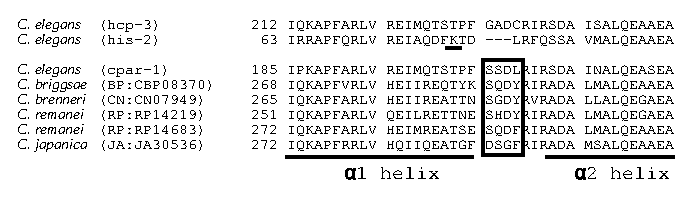
\includegraphics{Fig1}
\caption{Alignment of \protect\emph{Caenorhabditis} \protect\mbox{CENP--A} homologues showing
conservation of possible PIKK recognition site inserted within H3 structure. The major
\protect\emph{C\@. elegans} \protect\mbox{CENP--A} homologue (\protect\mbox{hcp--3}) and a canonical
H3 isoform (\protect\mbox{his--2}) with lysine 79 underlined are shown above.}
\label{fig:celegans}
\end{figure}

\newpage

\begin{figure}
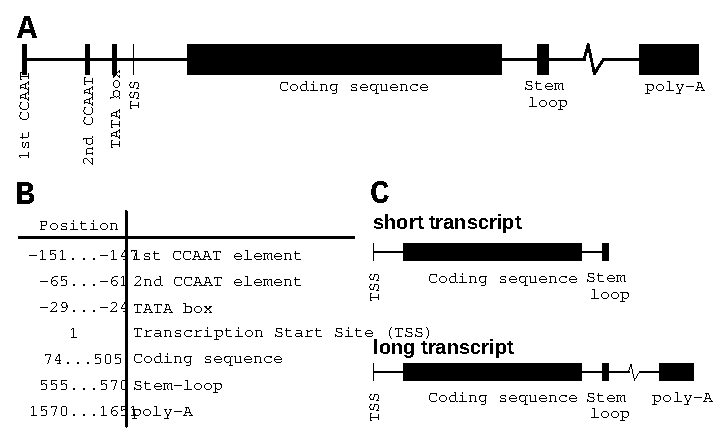
\includegraphics{Fig2}
\caption{H2AFX gene and transcripts. A.~Schematic of H2AFX gene region showing promoter and  3' mRNA
stabilizing elements. B.~Sequence coordinates of each element in H2AFX relative to transcription
start site\@. C.~Alternative transcripts of H2AFX\@. The short transcript  ($\approx$600\,bp in size) ends
in a stem--loop like canonical histones, whereas the long transcript ($\approx$1600\,bp in size) ends
in a poly--(A) tail.}
\label{fig:H2AFX}
\end{figure}

\newpage

\begin{figure}
\sidecaption
\includegraphics{Fig3}
\caption{Sequence logo of all human canonical H2A isoforms showing differences with H2AX below. The
4 residues changes from H2A to H2AX outside the C--terminal region are Gln\,6\,Thr, Thr\,16\,Ser, Asn\,38\,His
and Lys\,99\,Gly. Alignment of H2A genes was made usign edialign \protect\cite{Mor99} from EMBOSS
\protect\cite{RLB00} and WebLogo 3 \protect\cite{CHC+04}.}
\label{fig:H2AX-logo}
\end{figure}

\newpage

\begin{figure}
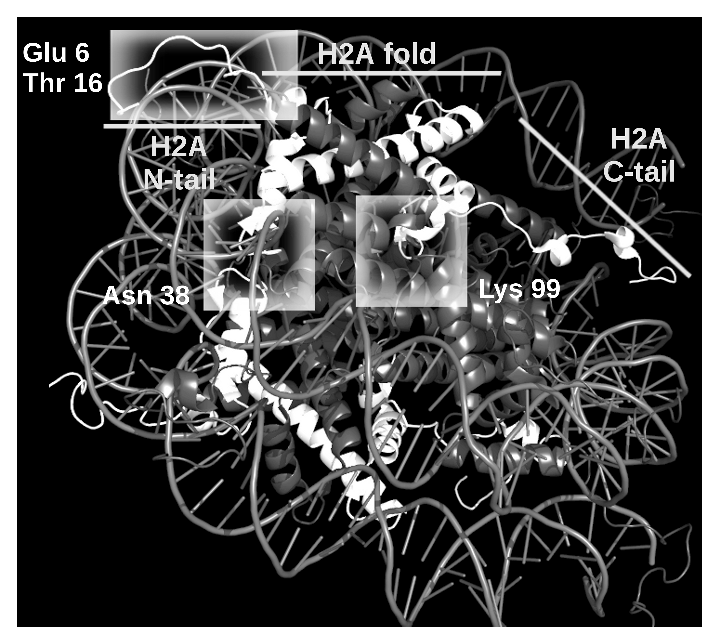
\includegraphics{Fig4}
\caption{Nucleosome structure highlighting differences between H2A and H2AX\@. H2A chain is
highlighted and white frames indicate the position of the residues that differ between the human
canonical H2A and H2AX\@. Image from PDB structure 1KX5 using PyMOL \protect\cite{DeL02}.}
\label{fig:H2AInNucleosome}
\end{figure}

\newpage

\begin{figure}
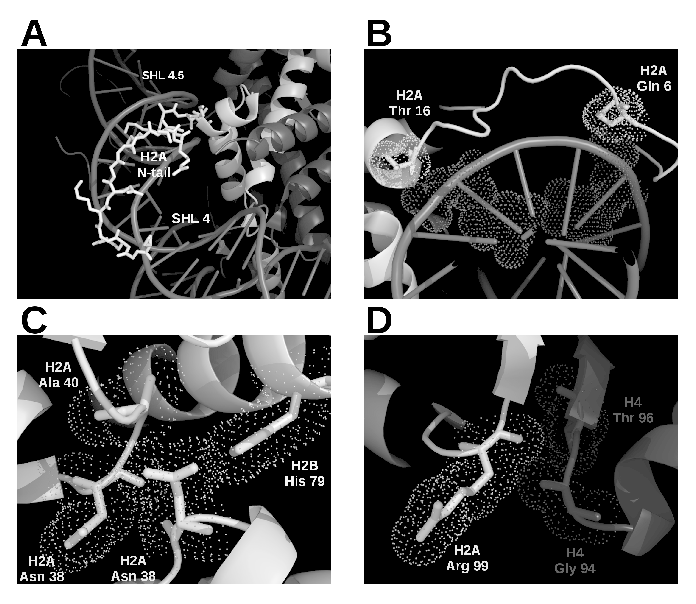
\includegraphics{Fig5}
\caption{Structural environment of H2A residues that differ from H2AX\@. The van der Waals surface
of differences and all residues within 5\AA\ are shown as a surface of dots over bond sticks. Image
from PDB structure 1KX5 using PyMOL \protect\cite{DeL02}. A.~H2A N--terminal tail encompassing H2AX
residues Thr\,6 and Ser\,16 passes across minor groove at superhelical location (SHL) 4.5\@. B.~Closeup
of H2A N--terminal tail minor groove association from A showing canonical H2A Gln\,6 and Thr\,16 which
become, respectively, Thr\,6 and Ser\,16 in H2AX\@. C.~Residues around H2A--H2A association in structure
showing interaction between paired Asn\,38 sidechains and adjacent residues. Canonical H2A Asn\,38 is
His\,38 in mammalian H2AX\@. D.~Environment around H2A Arg\,99 showing unusual absence of close packing.
Canonical H2A Arg\,99 is Gly\,99 in H2AX.}
\label{fig:framed}
\end{figure}

\newpage

\begin{figure}
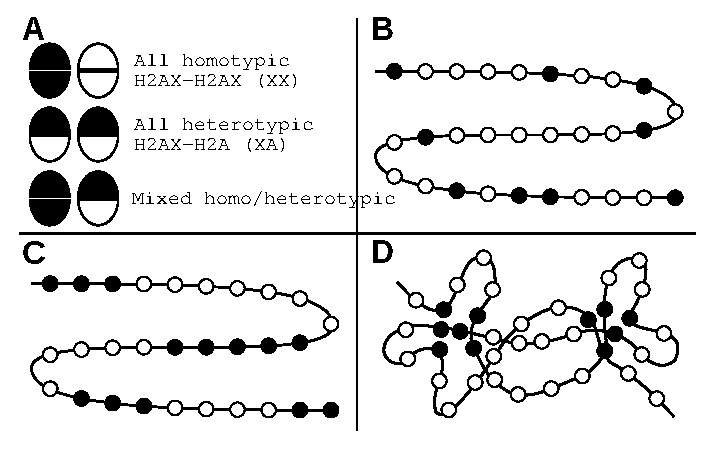
\includegraphics{Fig6}
\caption{H2AX distribution in the chromatin. A.~Schematic of possible H2AX homotypic, heterotypic and
mixed nucleosome combinations. Black semicircle represents H2AX--H2B dimer and white semicircle
represents H2A--H2B dimer. B.~Random incorporation of H2AX into nucleosomes would lead to a random
distribution of H2AX-containing nucleosomes. C.~Selective incorporation of H2AX into nucleosomes
would lead to ``islands'' of H2AX-containing nucleosomes. D.~Random incorporation of H2AX nucleosomes
could also lead to ``islands'' of H2AX nucleosomes by chromatin reorganization.}
\label{fig:H2AX-distribution}
\end{figure}

\newpage

\begin{figure}
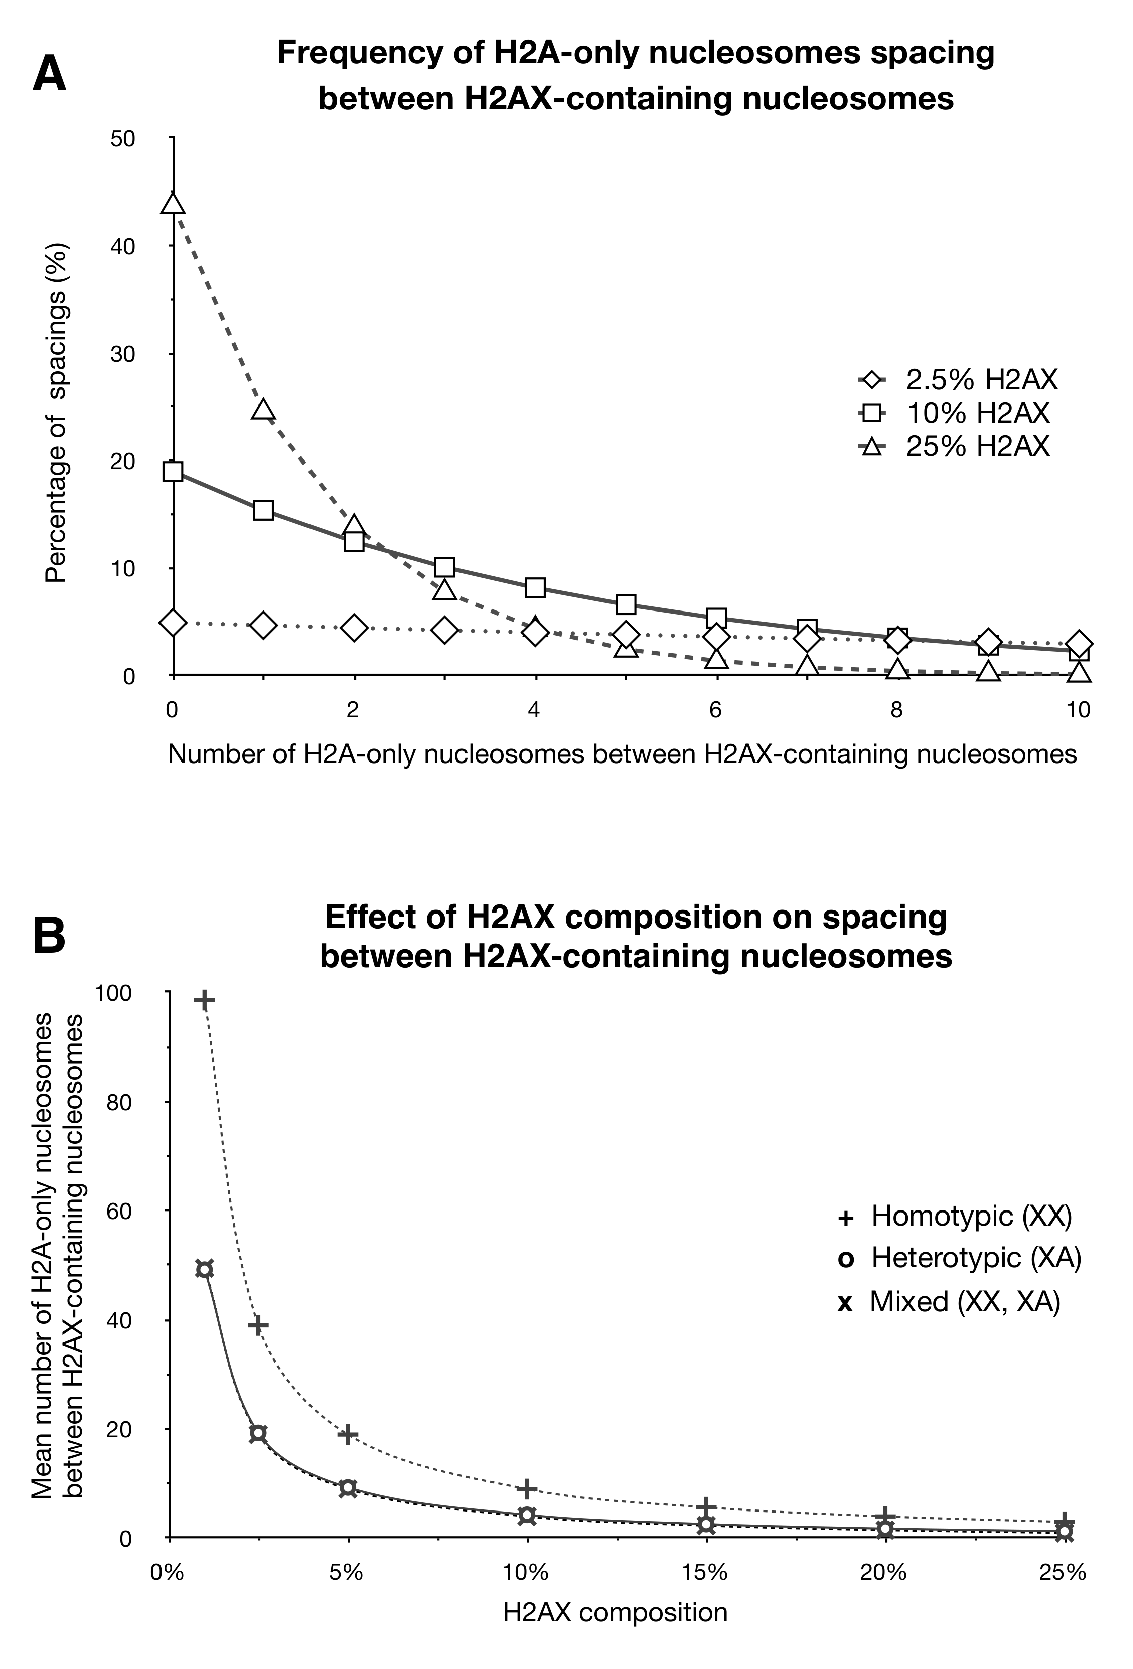
\includegraphics{Fig7}
\caption{Simulations of H2AX spacing distributions. A.~Distribution of spacings between instances of
H2AX for mixed population of homotypic and heterotypic nucleosomes at abundances of 2.5\% (dot),
10\% (solid) and 25\% (dashed) H2AX in total H2A pool. B.~Effect of abundance on mean H2AX spacing
for homotypic (H2AX--H2AX) only, heterotypic (H2AX--H2A) only, and mixed homotypic$+$heterotypic
nucleosome combinations.}
\label{fig:H2AX-graphs}
\end{figure}

\end{document}


